\section{Modificador}

El modificador que he utilizado ha sido el de \textit{Stretch}, muy similar a como el ejemplo del seminario, pero algo más refinado.

\bigskip

Este modificador lo que hace en la animación es aplastar el objeto cuando entra en contacto con el suelo y estirarse cuando se encuentra subiendo en el aire. Así se consigue dar la sensación de elasticidad en el objeto.

% foto de las diferencias entre aplastado y estirado
\begin{figure}[H]
    \centering 
	\begin{subfigure}[t]{0.45\textwidth}
	    \centering
	    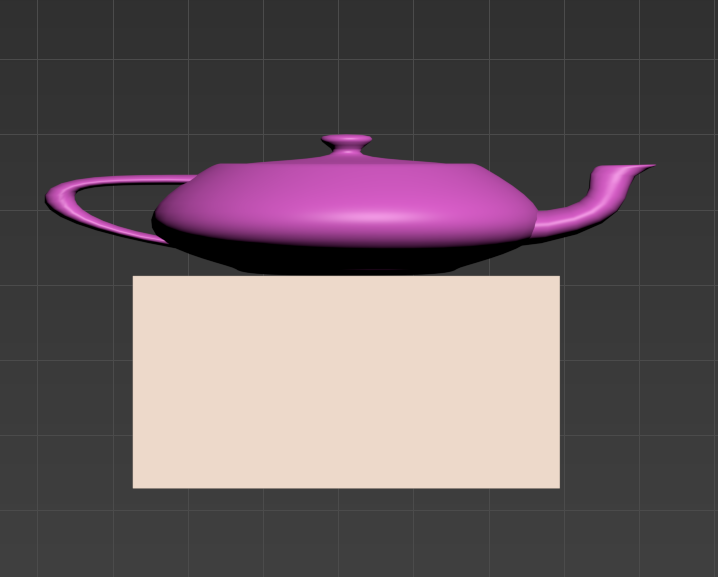
\includegraphics[width=\textwidth]{imagenes/aplastado.png}
        \caption{Objeto aplastado al máximo.}
    \end{subfigure}
    \hfill
	\begin{subfigure}[t]{0.45\textwidth}
	    \centering
	    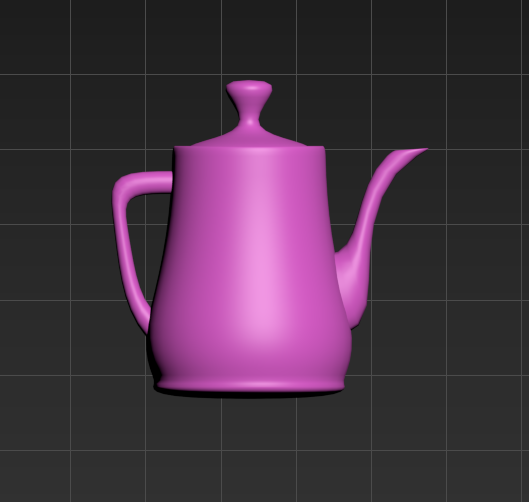
\includegraphics[width=\textwidth]{imagenes/estirado.png}
        \caption{Objeto estirado al máximo.}
    \end{subfigure}    
    \caption{Distintas formas aplicadas por el modificador.}
\end{figure}

Para implementarlo, he hecho que el objeto cuando comienza a subir, hasta llegar a un 15\% en la parábola interpolada, pase de estar aplastado a estirado completamente. Mientras que en los últimos 15\% de la parábola en la bajada, pasa de estar estirado completamente a aplastarse.

\bigskip

He necesitado realizar una interpolación lineal de los valores que toma el modificador \textit{Stretch} para que la animación sea fluida. La fórmula es: $f(t)=(1-t) \cdot ini + t \cdot fin$, donde ``ini'' representa la cantidad de estiramiento que presenta el objeto al inicio y ``fin'' representa la cantidad de estiramiento que presenta el objeto al final.

\bigskip

Además, al tener que realizarse la animación de estiramiento en el intervalo de interpolación [0, 0.15] y para aplastarse en el intervalo [0.85, 1], he necesitado mapear estos valores al intervalo [0, 1], para que el estiramiento y aplastamiento funcionen bien. Para ello, he creado una función \textit{Map Range Clamped}, con el mismo funcionamiento que la función con el mismo nombre en \textit{Unreal Engine}. Además, al ser \textit{clamped} permite que los valores nunca se saldrán del rango al ser evaluados por la función mapeadora.